% Greedy dual policy

In this section, we discuss the system model for function keep-alive, the goals and considerations for keep-alive policies, and present our caching-inspired greedy-dual policy. 

\noindent \textbf{System model:} 
We assume that each function invocation runs in its own container. 
%
A FaaS platform may use a cluster of physical servers, and forward the function invocation requests to different servers based on some load-balancing policy. 
Our aim is to investigate general keep-alive techniques that are independent of the load-balancing, and we therefore focus on \emph{server-level} policies. 
Even on a single server, a function can have multiple independent and concurrent instantiations, and hence containers.
Each function has its own container image and initialization code, and thus containers cannot be used by multiple functions. 
A function's containers are nearly identical in their resource utilization, since they are typically running the same function code.
When a function finishes execution, its container may be terminated, or be kept alive and ``warm'' for any future invocations of the same function. 
%
At any instant of time, each container is either running a function, or is being kept alive/warm. % (see Figure~\ref{fig:server}). 
%
Thus, server resources are consumed by running containers, and containers being kept alive in anticipation for future invocations. 


%Before invoking a function, users need to register it with the FaaS platform.  
%Registering typically entails providing information about which language the function is written in, the function body, and any initialization code that the function execution requires. 


% Figure with running, cached, and free, can be referenced here? 
\vspace*{\subsecspace}
\subsection{Policy Goals and Considerations}
\vspace*{\subsecspace}

The primary goal of keep-alive is to reduce the initialization and cold-start latency, by keeping functions alive for different durations based on their characteristics. 
% Servers that run these functions are heavily multiplexed, and run hundreds of short lived functions concurrently. %backend FaaS servers?
% too sudden 
Because servers run hundreds of short lived functions concurrently, keep-alive policies must be generalizable and yield high server utilization. 
%
Functions can have vastly different characteristics, and keep-alive polices must work efficiently in highly dynamic and diverse settings. % (Table~\ref{tab:workloads}). 
We have identified the following characteristics of functions that are the most pertinent for keep-alive policies.


The \textbf{initialization time} of functions can vary based on the code and data dependencies of the function.  
For example, a function for machine learning inference may be initialized by importing large ML libraries (such as TensorFlow, etc.), and fetching the ML model, which can be hundreds of megabytes in size and take several seconds to download. 
Functions also differ in terms of their \textbf{total running time}, which includes the initialization time and the actual execution time. 
Again, functions for deep-learning inference can take several seconds, whereas functions for HTTP servers and microservices are extremely short-lived (few milliseconds). 
The \textbf{resource footprint} of functions comprises of their CPU, memory, and I/O use, and also differs widely based on the application's requirements. 
Finally, functions have different \textbf{popularities}, and are called with different rates. Some functions may be invoked several times a second, whereas other functions may only be invoked rarely (if they are used to serve a very low-traffic web-site, for instance). 

% \begin{figure}[t]
%   \centering
%   \vspace*{\myfigspace}
%   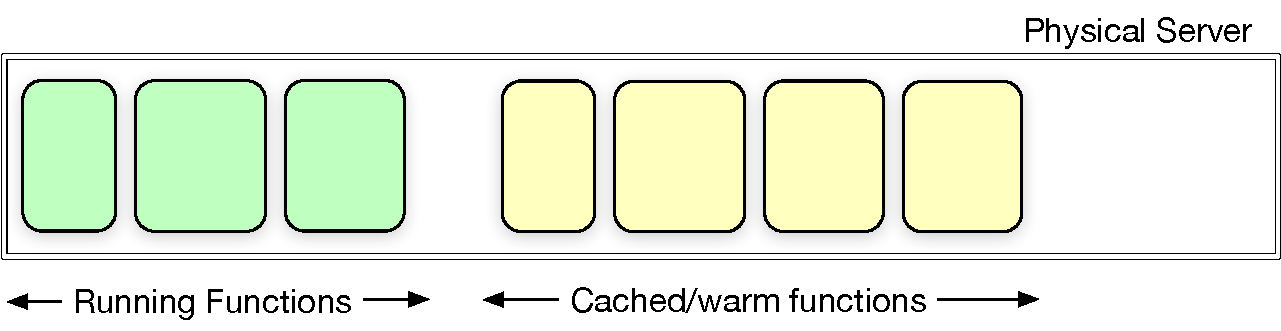
\includegraphics[width=0.4\textwidth]{../graphs/faas.pdf}
%   \vspace*{\myfigspace}
%   \label{fig:runwarm}
%   \caption{Server resources are consumed by running and warm containers.}
%     \vspace*{\myfigspace}
% \end{figure}


Because server resources are finite, it is important to prioritize functions that should be kept alive, based on the aforementioned characteristics. 
%
A function which is not popular and is unlikely to be called again in the near future, sees little benefits from keep-alive. 
In fact, keeping such functions alive consumes valuable server computing resources for no gain in efficiency. %energy.. hmm
Thus, keep-alive policies should prioritize popular functions. 
%
Similarly, the resource consumption of the functions is also important: since keeping large-footprint functions alive is more expensive than smaller functions, smaller functions should be preferred and kept alive for longer. 
%
Finally, functions can also be prioritized based on their initialization overhead, since it is effectively wasted computation.

% This paragraph is key. Different priorities and there is no one single ranking scheme for keepalive... 
The problem of designing keep-alive policies is complicated by the fact that functions may have vastly different keep-alive priorities for the different characteristics.
Consider a function with a large memory footprint (like those used in ML inference), high initialization overhead, and a low popularity.
Such a function should have a low priority due to its size, high priority due to large initialization overhead, and a low priority due to its low popularity.
Thus, keep-alive policies must carefully balance all the different function characteristics and prioritize them in a coherent manner.


FaaS frameworks such as OpenWhisk, keep all functions alive for a \emph{constant} period of time (30 minutes), or use LRU-based termination. 
%
These policies are agnostic to different function characteristics such as resource footprint and initialization overheads, and only loosely capture popularity. 
%
A more principled approach is needed, which we provide next. 


% \textbf{A small example should be described here with actual function characteristics and effect of const-TTL.}

% Thus, functions may have different keep-alive 

% Keep-alive policies can have a significant impact based on function characteristics, and have many different tradeoffs. 

% Since functions are executed 

% %Each of these functions have different characteristics, and smart keep-alive policies must run all 



% While keeping the containers alive can reduce the function execution latency, the running containers consume resources, which reduces the number of concurrent functions that can be executed. 

% We assume a single physical server runs many functions concurrently. 

% The number of functions that can be executed concurrently depends on the resource availability on the server.
% %
% Containers that are kept alive consume resources that can be used to run additional functions, and thus reduce the effective server utilization.

% Keep-alive thus imposes an important tradeoff. 
% %
% Policies must be cognizant of different factors.
% %
% The cold start (i.e., initilization) overhead, the total execution time, the resource footprint (i.e., memory occupied), and the frequency of the function invocation. 
% %

% Constant keep-alive policies (for 30 minutes) do not consider the resource footprints, nor do they take into account the benefits of warming for different functions.
% %
% For instance, given two containers close to their time out, we should ideally prefer the one with high cold-start overhead so that the work is not lost.

% Similarly, resource footprint is another major factor. Higher footprint containers should be evicted earlier.

% Ofcourse we need to consider multiple factors: footprint, access frequency, cold-start overhead, and size.
% %
% Optimizing for server-times 

% Our primary insight is that principled keep-alive policies can be derived if we look at this as a caching problem. 
% %
\vspace*{\subsecspace}
\subsection{Keep-alive is Equivalent to Caching}
\vspace*{\subsecspace}

Formulating a keep-alive policy that balances the characteristics of all competing functions, seems daunting. 
\emph{The central insight of this paper is that keeping functions alive is equivalent to keeping objects in a cache.} 


%The problem of what functions to keep alive and for how long, is equivalent to what objects to cache. 
Keeping a function alive reduces its effective execution latency, in the same way as caching an object reduces its access latency. 
When all server resources are fully utilized, the problem of which functions \emph{not} to keep alive is equivalent to which objects to \emph{evict} from the cache. 
The high-level goal in caching is to improve the distribution of object access times, which is analogous to our goal of reducing the effective function latencies. 


This caching analogy provides us a framework and tools for understanding the tradeoffs in keep-alive policies, and improving server utilization. 
%The problem of cache eviction in object caching is a thoroughly studied for a wide range of constraints, systems, and environments. 
Caching has been studied in wide range of contexts and many existing caching techniques can be applied and used for function keep-alive. 
Our insight is that we can use classic observations and results in object caching to formulate equivalent keep-alive policies, that can provide us with well-proven and sophisticated starting point for understanding and improving function keep-alive.  





% We assume that each function in its own container.
% When the function is ``registered'', this container image is created.
% Multiple concurrent invocations to the same function are possible, but each invocation is in its own container.
% Containers are in one of two states. Either running the function, or are idling when they are being kept warm. 
% When a function is called by the user, if a corresponding container is ``free'', then it is used to run the function.
% Otherwise, a new container is instantiated.

% When a container is launched, the initilization code runs.
% Depending on the application and the FaaS platform, the amount of initilization can be different.
% For example, a truly ``stateless'' function will include all required dependencies on every invocation.
% In any case, there is some initilization and start-up overhead, which consumes 


% While any caching/eviction algorithm can be used with the help of this analogy after the mapping, the algorithm must be cognizant of the different resource footprints and access frequencies and execution latencies of different functions.
% %
% The greedy dual approach is a good mapping, which we use below. 

\vspace*{\subsecspace}
\subsection{Greedy-Dual Keep-Alive Policy}
\vspace*{\subsecspace}

While many caching techniques can be applied to the function keep-alive policies, we now present one such caching-inspired policy that is simple and yet captures all function characteristics and their tradeoffs.
Our policy is based on Greedy-Dual-Size-Frequency object caching~\cite{gdsf}, which was designed for caches with objects of  different sizes, such as web-caches. 
Classical caching policies such as LRU or LFU do not consider object sizes, and thus cannot be completely mapped to the keep-alive problem where the resource footprint of functions is an important characteristic. 
As we shall show, the Greedy-Dual-Size-Frequency approach provides a general framework to design and implement keep-alive policies that are cognizant of the  frequency and recency of invocations of different functions, their initialization overheads, and sizes (resource footprints). 



Fundamentally, our keep-alive policy is a function \emph{termination} policy, just like caching focuses on eviction policies. 
%
Our policy is resource conserving: we keep the functions warm whenever possible, as long as there are available server resources.
%
This is a departure from current constant time-to-live policies implemented in public clouds, that are \emph{not} resource conserving, and may terminate functions even if resources are available to keep them alive for longer. 

%We assume that each functions is deployed in a container, and o
Our policy decides which container to terminate if a new container is to be launched and there is not enough resource availability.
%
The total number of containers (warm + running) is constrained by the total server physical resources (cpu and memory). 
%
Intuitively, our termination policy computes a ``priority'' for each container based on the cold-start overhead and resource footprint, and terminates the container with the lowest priority.
%
%Below, we describe our termination policy in detail.


%\noindent \textbf{Execution model.}
%Assume that there are $n$ different functions.
%
%We assume that each function runs in its own container.
%
%Each function can have multiple independent and concurrent instantiations, and hence containers. 
%
%At any instant of time, each container is either running a function, or is being kept alive/warm. 
%

%What is the point of this? 
%Assume that a  function $i$ has a initialization or startup time of $s_i$. 
%Once initialized, the running time of the function is  $r_i$, and thus total running time for the cold-start case is $s_i + r_i = T_i$.  
%When executing on a warm container, the time is simply $w_i$.
%


%Let $m_i$ be the memory footprint of the function.


%The total number of containers (warm + running) is constrained by the total server physical resources (cpu and memory). 
%Each container has a resource footprint, which we also call the \emph{size} of the container, denoted by $\mathbf{d_i}$.
%The size may be a multi-dimensional resource vector comprising of the CPU, memory, and I/O resources used by the running or warm container.
%In most scenarios, the number of containers that can run is limited by the physical memory availability, since CPUs can be multiplexed easily, and memory swapping can result in severe performance degradation.
%Thus for ease of exposition, we can consider only the container \emph{memory} use as the size, instead of a multi-dimensional vector. 


\noindent \textbf{Priority Calculation.} 
Our greedy dual policy is based on greedy dual caching~\cite{gdsf}. 
%
For each container, we assign a \emph{keep-alive priority}, which is computed based on the frequency of function invocation, its running time, and its size. 
%
The priority is given by:   \vspace*{-7pt}
\begin{equation}
  \vspace*{-7pt}
  \text{Priority} = \text{Clock} + \frac{\text{Freq} \times \text{Cost}} {\text{Size}}
    \label{eq:prio-prop}
\end{equation}
%
% 

On every function invocation, if a warm container for the function is available, it is used, and its frequency and priority are updated.
Reusing a warm container is thus a ``cache hit'', since we do not incur the initialization overhead. 
%
When a new container must be launched if there are insufficient resources, then containers are terminated based on their priority order---lower priority containers are terminated first. 
%
We now explain the intuition behind each parameter in the priority calculation:



\noindent \textbf{Clock} is used to capture the recency of execution.
%
We maintain a ``logical clock'' per server.
%
Each time a container is used, the server clock is assigned to the container and the priority is updated. 
%
Thus, containers that are not recently used will have smaller clock values (and hence priorities), and will be terminated before more recently used containers. 

The logical clock is updated only when a container is terminated. 
Containers are terminated only if there are insufficient resources to launch the new container and if existing warm containers cannot be used.  
%
Specifically, if a container  $j$ is terminated (because it has the lowest priority), then $\text{Clock} = \text{Priority}_j$.
All subsequent uses of other, non-terminated containers then use this clock value for their priority calculation.
%
In some cases, \emph{multiple} containers may need to be terminated to make room for new containers.
%
If $E$ is the set of these terminated containers, then $\text{Clock} = \max_{j \in E}{\text{Priority(j)}}$

We note that the priority computation is on a per-container basis, and containers of the same function share some of the attributes (such as size, frequency, and cost). 
However, the clock attribute is updated for each container individually.
This allows us to evict the oldest and least recently used container for a given function in order to break ties. 



\noindent \textbf{Frequency} is the number of times a given function is invoked.
%
A given function can be executed by multiple containers, and frequency denotes the \emph{total} number of function invocations across all of its containers. 
%
The frequency is set to zero when all the containers of a function are terminated.
%
The priority is proportional to the frequency, and thus more frequently executed functions are kept alive for longer. 
%
%This is a departure from object caching, where each object is distinct. In our case, because of concurrent executions of functions, multiple containers for the same function may exist, and we thus take into account all the 
%


\noindent \textbf{Cost} represents the termination-cost, which is equal to the initialization time, i.e., $s_i$. 
%
This captures the benefit of keeping a container alive and the cost of a cold-start. 
%
% There are other cost formulations also, such as $c/T$ etc that capture the ratio, that yield different policies.
The priority is thus proportional to the initialization overhead of the function. 





\noindent \textbf{Size} is the resource footprint of the container. 
%
%If we only care about the memory size, then we can simply use a single dimensional metric $m_i$ to denote the size.
%
The priority is inversely proportional to the size, and thus larger containers are terminated before smaller ones. 
%
We can use multi-dimensional resource vectors to represent the size, in which case we convert them to scalar representations by using the existing formulations from multi-dimensional \emph{bin-packing.}
%
For instance, if the container size is $\mathbf{d_i}$, then the size can be represented by the magnitude of the vector $||\mathbf{d_i}||$.
%
Other size representations can also be used.
A common technique is to normalize the container size by the physical server's total resources ($\mathbf{a}$), and then compute the size as $\sum_j \frac{d_j}{a_j}$ where $d_j, a_j$ are the container size and total resources of a given type (either CPU, memory, I/O) respectively.
%
Cosine similarity between $\mathbf{d}$ and $\mathbf{a}$ can also be used, as is widely used in multi-dimensional bin-packing. 

In most scenarios, the number of containers that can run is limited by the physical memory availability, since CPUs can be multiplexed easily, and memory swapping can result in severe performance degradation.
Thus for ease of exposition and practicality, we can consider only the container \emph{memory} use as the size, instead of a multi-dimensional vector. 



%


%







%%% Local Variables:
%%% mode: latex
%%% TeX-master: "paper"
%%% End:
